% ----------------------------------------------------
% Methodology
% ----------------------------------------------------
\documentclass[class=report,11pt,crop=false]{standalone}
\input{../Style/ChapterStyle.tex}
\makenoidxglossaries

\newacronym{fm}{FM}{frequency modulation}
\newacronym{lora}{LoRa}{Long Range}
\newacronym{iot}{IOT}{Internet of Things}
\newacronym{fsk}{FSK}{Frequency Shift Keying}
\newacronym{chirp}{CHIRP}{Compressed High Intensity Radar Pulse}
\newacronym{atps}{ATPs}{Acceptance Test Protocols}
\newacronym{hal}{HAL}{Hardware Abstraction Layer}
\newacronym{oled}{OLED}{Organic Light Emitting Diode}
\newacronym{rssi}{RSSI}{Received Signal Strength Index}
\newacronym{uart}{UART}{Universal Asynchronous Receive and Transmit}
\newacronym{usb}{USB}{Universal Serial Bus}
\newacronym{css}{CSS}{Chirp Spread Spectrum}
\newacronym{i2c}{I2C}{Inter-Integrated Circuit}
\newacronym{spi}{SPI}{Serial Peripheral Interface}
\newacronym{gps}{GPS}{Global Positioning System}
\newacronym{nmea}{NMEA}{National Marine Electronics Association}
\newacronym{mac}{MAC}{Media Access Control}
\newacronym{sf}{SF}{Spreading Factor}
\newacronym{arr}{ARR}{Auto Reload Register}
\newacronym{sdr}{SDR}{Software Defined Radio}
\newacronym{pcb}{PCB}{Printed Circuit Board}
\newacronym{fdm}{FDM}{Frequency Division Multiplexing}


\newacronym{radar}{RADAR}{Radio Detection and Ranging}
\newacronym{ofdm}{OFDM}{Orthogonal Frequency Division Multiplexing}
\newacronym{tdm}{TDM}{Time Division Multiplexing}
\newacronym{tdma}{TDMA}{Time Division Multiple Access}
\newacronym{att}{AT\&T}{American Telephone and Telegraph Company}
\newacronym{usrp}{USRP}{Universal Software Radio Peripheral}
\newacronym{uct}{UCT}{University of Cape Town}


\begin{document}
% ----------------------------------------------------
\chapter{Methodology \label{ch:methodology}}
Now that the design of the prototype transmission and receiver circuits has been completed, the methodology used in the design of the experiments with the transmission and receiver circuit must be examined and explained. The design of the experiments was thought out over some time and after some discussions with my supervisor.

\section{Research Design and Approach}
After analysis of the overall project, it was determined that the most pertinent question that I had to answer, was exactly what LoRa parameters made for the best transmission settings for a mock weather balloon setup. That is why I designed the initial prototypes of the transmission and receiver circuits in the first place. The LoRa module has the following parameters which can be adjusted according to the user's needs. These settings apply to whatever frequency the LoRa module is currently operating at, be that 433MHz exactly or a slight deviation to a higher or lower frequency. For my experiments, I decided it was best to keep my centre frequency at exactly 433MHz. Other than the centre frequency, the other parameters which a user is able to customize for the SX1278 LoRa module can be seen below in table \ref{tab:sx1278parametersandoptions}.

\begin{table}[H]
\centering
\begin{tabular}{|c|c|}
\hline
\textbf{Parameter} & \textbf{No. of Different Options} \\ \hline
Spreading Factor   & 6                                 \\ \hline
Bandwidth          & 10                                \\ \hline
Coding Rate        & 4                                 \\ \hline
Power Gain         & 4                                 \\ \hline
\end{tabular}
\caption{Various parameters and their options available for the SX1278 LoRa module}
\label{tab:sx1278parametersandoptions}
\end{table}

This table highlights how if I were to test each permutation of the available LoRa settings, then I would need to perform $6\times10\times4\times4=960$ tests. This is a fairly unrealistic number of tests to perform, seeing as I would need at least 10-15 seconds of recording of data per permutation of LoRa settings, with 960 tests, it would take between 2.67 and 4 hours to perform one communication test. It was therefore decided that the power gain would be set to a maximum value of 20dB and that the coding rate would be set to the most minimal value of 4/5. The argument for setting the power value as high as possible is that the aim of the project is to maximise the transmission distance of the LoRa module, and setting the output power of the LoRa transmitter to a maximum value would aid in this goal. Setting the coding rate to a value of 4/5 made sense because as you increase the coding rate to values such as 4/6, 4/7, and 4/8, the LoRa module adds more redundancy check data per packet of payload data for integrity purposes. It was therefore decided that since the goal of the project was to maximise range, the coding rate should be kept at 4/5, since this adds the least amount of extra data onto the transmission, therefore allowing for more transmission modes to be utilised, since having less data to send unlocks the ability to use lower data rate transmission setting combinations on the LoRa module. After making these changes, the number of permutations of the LoRa settings is $6\times10\times1\times1=60$. This dramatically reduces the overall number of tests that need to be performed, while still keeping the experiments as realistic as possible with regards to the real-world scenario of a weather balloon. 

With the goal in mind of determining the best parameters for the LoRa module for long-range tests, it was decided that multiple tests of the LoRa transmission and receiver circuits should be carried out at varying distances away from each other while operating in various modes. These modes would be labelled from 1-60 and would each correspond to a specific LoRa setting combination. The various modes and the corresponding setting combinations can be seen in table \ref{tab:testingmodepermutations} below. 

\begin{table}[H]
\centering
\begin{tabular}{|c|c|c|c|c|c|c|}
\cline{1-3} \cline{5-7}
\textbf{Mode} & \textbf{\begin{tabular}[c]{@{}c@{}}Spreading\\ Factor\end{tabular}} & \textbf{Bandwidth (kHz)} & \textbf{} & \textbf{Mode} & \textbf{\begin{tabular}[c]{@{}c@{}}Spreading\\ Factor\end{tabular}} & \textbf{Bandwidth (kHz)} \\ \cline{1-3} \cline{5-7} 
1             & 7                                                                   & 7.8                      &           & 31            & 10                                                                  & 7.8                      \\ \cline{1-3} \cline{5-7} 
2             & 7                                                                   & 10.4                     &           & 32            & 10                                                                  & 10.4                     \\ \cline{1-3} \cline{5-7} 
3             & 7                                                                   & 15.6                     &           & 33            & 10                                                                  & 15.6                     \\ \cline{1-3} \cline{5-7} 
4             & 7                                                                   & 20.8                     &           & 34            & 10                                                                  & 20.8                     \\ \cline{1-3} \cline{5-7} 
5             & 7                                                                   & 31.25                    &           & 35            & 10                                                                  & 31.25                    \\ \cline{1-3} \cline{5-7} 
6             & 7                                                                   & 41.7                     &           & 36            & 10                                                                  & 41.7                     \\ \cline{1-3} \cline{5-7} 
7             & 7                                                                   & 62.5                     &           & 37            & 10                                                                  & 62.5                     \\ \cline{1-3} \cline{5-7} 
8             & 7                                                                   & 125                      &           & 38            & 10                                                                  & 125                      \\ \cline{1-3} \cline{5-7} 
9             & 7                                                                   & 250                      &           & 39            & 10                                                                  & 250                      \\ \cline{1-3} \cline{5-7} 
10            & 7                                                                   & 500                      &           & 40            & 10                                                                  & 500                      \\ \cline{1-3} \cline{5-7} 
11            & 8                                                                   & 7.8                      &           & 41            & 11                                                                  & 7.8                      \\ \cline{1-3} \cline{5-7} 
12            & 8                                                                   & 10.4                     &           & 42            & 11                                                                  & 10.4                     \\ \cline{1-3} \cline{5-7} 
13            & 8                                                                   & 15.6                     &           & 43            & 11                                                                  & 15.6                     \\ \cline{1-3} \cline{5-7} 
14            & 8                                                                   & 20.8                     &           & 44            & 11                                                                  & 20.8                     \\ \cline{1-3} \cline{5-7} 
15            & 8                                                                   & 31.25                    &           & 45            & 11                                                                  & 31.25                    \\ \cline{1-3} \cline{5-7} 
16            & 8                                                                   & 41.7                     &           & 46            & 11                                                                  & 41.7                     \\ \cline{1-3} \cline{5-7} 
17            & 8                                                                   & 62.5                     &           & 47            & 11                                                                  & 62.5                     \\ \cline{1-3} \cline{5-7} 
18            & 8                                                                   & 125                      &           & 48            & 11                                                                  & 125                      \\ \cline{1-3} \cline{5-7} 
19            & 8                                                                   & 250                      &           & 49            & 11                                                                  & 250                      \\ \cline{1-3} \cline{5-7} 
20            & 8                                                                   & 500                      &           & 50            & 11                                                                  & 500                      \\ \cline{1-3} \cline{5-7} 
21            & 9                                                                   & 7.8                      &           & 51            & 12                                                                  & 7.8                      \\ \cline{1-3} \cline{5-7} 
22            & 9                                                                   & 10.4                     &           & 52            & 12                                                                  & 10.4                     \\ \cline{1-3} \cline{5-7} 
23            & 9                                                                   & 15.6                     &           & 53            & 12                                                                  & 15.6                     \\ \cline{1-3} \cline{5-7} 
24            & 9                                                                   & 20.8                     &           & 54            & 12                                                                  & 20.8                     \\ \cline{1-3} \cline{5-7} 
25            & 9                                                                   & 31.25                    &           & 55            & 12                                                                  & 31.25                    \\ \cline{1-3} \cline{5-7} 
26            & 9                                                                   & 41.7                     &           & 56            & 12                                                                  & 41.7                     \\ \cline{1-3} \cline{5-7} 
27            & 9                                                                   & 62.5                     &           & 57            & 12                                                                  & 62.5                     \\ \cline{1-3} \cline{5-7} 
28            & 9                                                                   & 125                      &           & 58            & 12                                                                  & 125                      \\ \cline{1-3} \cline{5-7} 
29            & 9                                                                   & 250                      &           & 59            & 12                                                                  & 250                      \\ \cline{1-3} \cline{5-7} 
30            & 9                                                                   & 500                      &           & 60            & 12                                                                  & 500                      \\ \cline{1-3} \cline{5-7} 
\end{tabular}
\caption{Different testing modes and their corresponding LoRa parameter permutations}
\label{tab:testingmodepermutations}
\end{table}

The performance of each of the different modes listed above would be determined by the average RSSI value of each packet received on each specific mode by the receiver circuit. The different LoRa modes have to be applied to the transmitter and receiver circuits for the system to operate properly. This is why the display and control modules were such a critical aspect of the design of the overall system as highlighted in chapter \ref{ch:systemdesign}. The people operating the transmission and receiver modules needed to be able to precisely control the Lora settings, and this is what the various operating modes allow for.

To keep all the tests performed consistent with each other, it was decided that the packet that would be transmitted during the testing phase would be four bytes in length. This provides a good base packet size, with which the data on the performance of the system can be extrapolated out to larger packet sizes. This was also done with the goal in mind of the overall system sending out the required data in a manner that has the overall packet broken up into smaller chunks to be sent. As can be seen in listing \ref{lst:sensormodulevalidation}, a full packet of data can be up to 61 characters in length. Therefore, if a full packet were to be transmitted with this scheme of sending four bytes of data at a time, then 15 LoRa transmissions would need to occur for each full packet of data. Whether or not this idea of breaking up the larger data packet into smaller chunks was favourable is discussed more in section \ref{sec:optimalpacketstructure} later on.

Based on all this previous information, I proposed the following tests to help determine the best LoRa parameters for long-range transmission.
\begin{enumerate}
    \item \textbf{Test 1}: Same room test. This test would give a very quick overview of the performance of the LoRa transmission and receive circuits. Since the transmission circuit and the receiver circuit would be placed so close together, I didn't expect to see any drastic changes in the performance of the system as the various modes were iterated through.
    \item \textbf{Test 2}: 100m test. This test would be the first test performed with a significant distance between the transmitter and receiver circuit and will show how the system performs over a short distance.
    \item \textbf{Test 3}: 300m test. This test would simply add on to the 100m test, and give more data to evaluate the performance of the system.
    \item \textbf{Test 4}: 500m test. This test would conclude the "medium" range tests.
    \item \textbf{Test 5}: 20km test. This test would constitute the long-range testing element of the system. This test would hopefully shine a light on the performance of the system at a more realistic distance that might be experienced with an actual weather balloon system's base station having to pick up a transmission signal.
\end{enumerate}

The idea of the first four tests is that they could be used to model the performance of the system over larger distances. Therefore, these first tests would be critical in helping to build an understanding of the initial performance of the system. The long-range test would confirm whether or not the understanding gained from the shorter-range tests carried through to the long-range test. 

\section{Data Collection}\label{sec:datacollection}
To perform the data collection required for the tests, at least two people are required to operate the overall system. One person needs to be with the transmitter module, and another person needs to be with the receiver module. In the experimental setup which I used, I was always the individual operating the receiver module as this gave me the ability to record the necessary data for processing. The two operators of their respective systems would need to be in constant communication to allow for the proper setting of the modes that were being tested. This was achieved using the cellular data network that exists in South Africa. The two operators simply called each other using the data network and were able to properly synchronise the modes on their respective modules. A diagram of the initial idea of the setup can be seen below in figure \ref{fig:datacollectiondiagram}.

\begin{figure}[H]
    \centering
    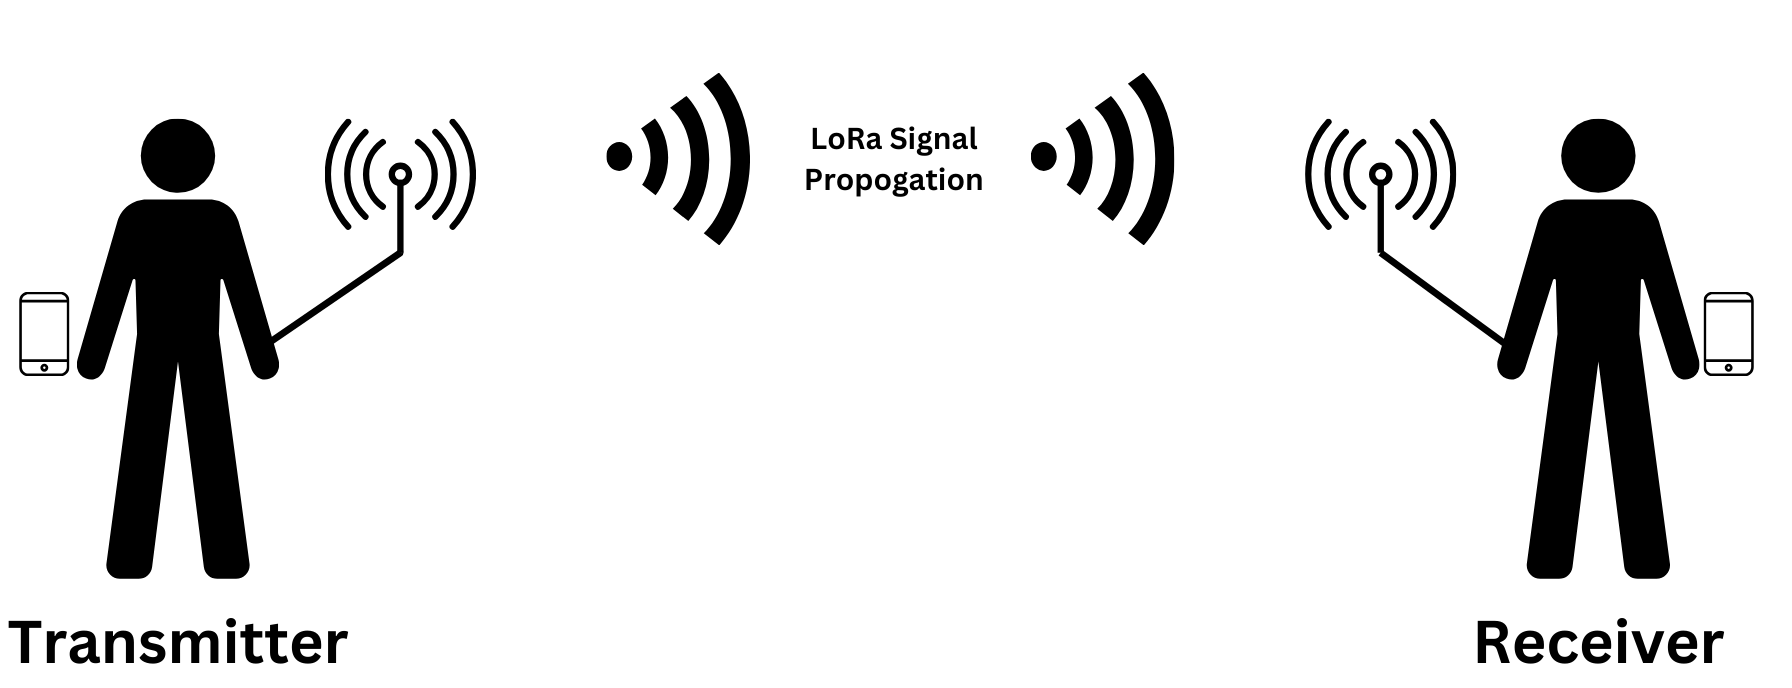
\includegraphics[width=0.6\linewidth]{../Images/dataCollectionDiagram.png}
    \caption{Diagram of Data Collection Process}
    \label{fig:datacollectiondiagram}
\end{figure}

The operator at the receiver side of the system needs to have access to a portable computer that has a USB port available. This is necessary because the receiver circuit gets its power through the onboard micro-USB port, unlike the transmitter circuit which gets its power from its onboard battery module. 

The operator of the receiver circuit also needs to have software loaded onto their computer that gives them the ability to read serial output from the built-in UART to USB adaptor on the ESP32-WROOM-32D microcontroller. The software that I used for this was SerialTools\footnote{The SerialTools software is a Macintosh-specific piece of software that can be found \href{https://apps.apple.com/us/app/serialtools/id611021963?mt=12}{here}.}. An alternative piece of software that could be used for Windows users is Putty\footnote{Putty is a Windows-specific application and can be found \href{https://www.putty.org}{here}.}.

After the required software to monitor the serial output of the receiver has been installed, the testing can begin. The process of data collection would follow the following steps.
\begin{enumerate}
    \item \textbf{Step 1}: Position the two modules at the required distance away from each other for their specific test that is taking place.
    \item \textbf{Step 2}: Place the antennas for the circuit at a height of more than 1 metre above the ground, on a secure mounting platform. 
    \item \textbf{Step 3}: Open up a communication channel between the two operators of the transmission and receiver circuit respectively. This communication channel must preferably be a voice chat between the two operators.
    \item \textbf{Step 4}: Power on the transmitter and receiver circuit. Each circuit will initialise in testing mode 1.
    \item \textbf{Step 5}: Wait for a few packets to transmit and receive on each mode, and then, over the voice call link, decide to change the operation mode to the next mode. If packets are not being received, wait at least 15-20 seconds before changing to the next mode.
    \item \textbf{Step 6}: Repeat Step 5 until all 60 modes have been iterated through.
    \item \textbf{Step 7}: After all the data has been captured on the serial monitor program of choice, copy the raw output of the serial monitor into a text editor of choice and save it as the raw data for the specific test performed.
\end{enumerate}

The above steps can then be repeated for each test that is performed at the various distances between the transmitter and receiver. 

\section{Shorter Range Tests}
For the shorter-range tests, which I have defined as the same room, 100m, 300m, and 500m tests, it was decided that the \gls{uct} rugby fields would be utilised as a testing ground. This was decided because the UCT rugby fields provide a wide open, and most importantly, flat space to do the required testing. It is important that the testing space be flat to create an accurate testing environment to simulate the line-of-site that would be experienced in the real world between a weather balloon radiosonde transmitter and the base station receiver. 

To get the testing started, the same room test was performed. This was done by placing the transmitter and receiver circuits next to each other and performing the required testing of the various modes. The next tests that were performed were the 100m, 300m, and 500m rugby field tests. In figure \ref{fig:shortrangerugbyfieldtests} below, a distance map can be seen of the three rugby field tests that were performed. These images show the distance between the transmitter module and the receiver module for each of the three tests performed on the rugby field.

\begin{figure}[H]
    \centering
    
    \begin{subfigure}[b]{0.3\textwidth}
        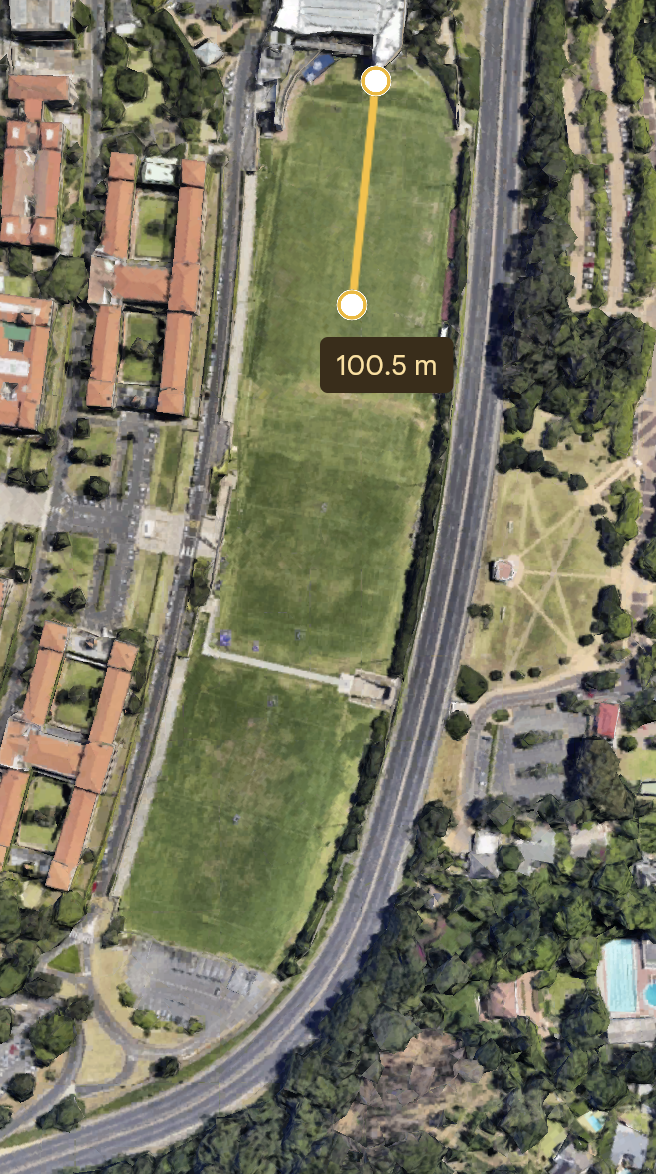
\includegraphics[width=\textwidth]{../Images/shortRangeTests/100mTestGoogleEarth.png}
        \caption{100m Test}
        \label{fig:100mtestgoogleearth}
    \end{subfigure}
    \hfill
    \begin{subfigure}[b]{0.3\textwidth}
        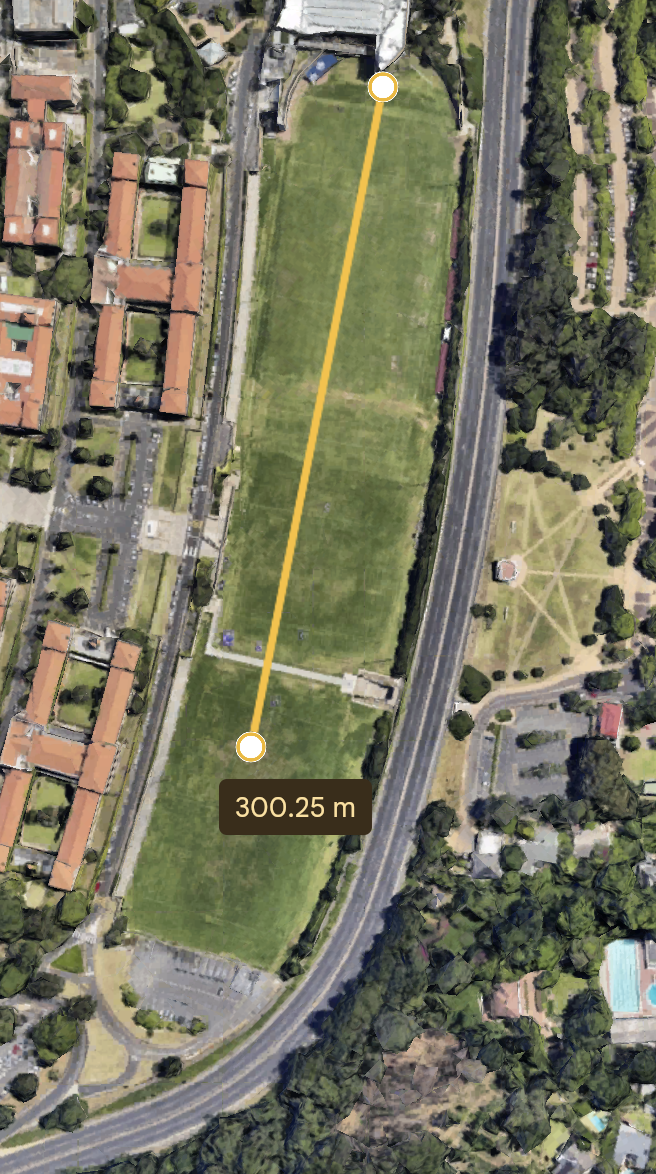
\includegraphics[width=\textwidth]{../Images/shortRangeTests/300mTestGoogleEarth.png}
        \caption{300m Test}
        \label{fig:300mtestgoogleearth}
    \end{subfigure}
    \hfill
    \begin{subfigure}[b]{0.3\textwidth}
        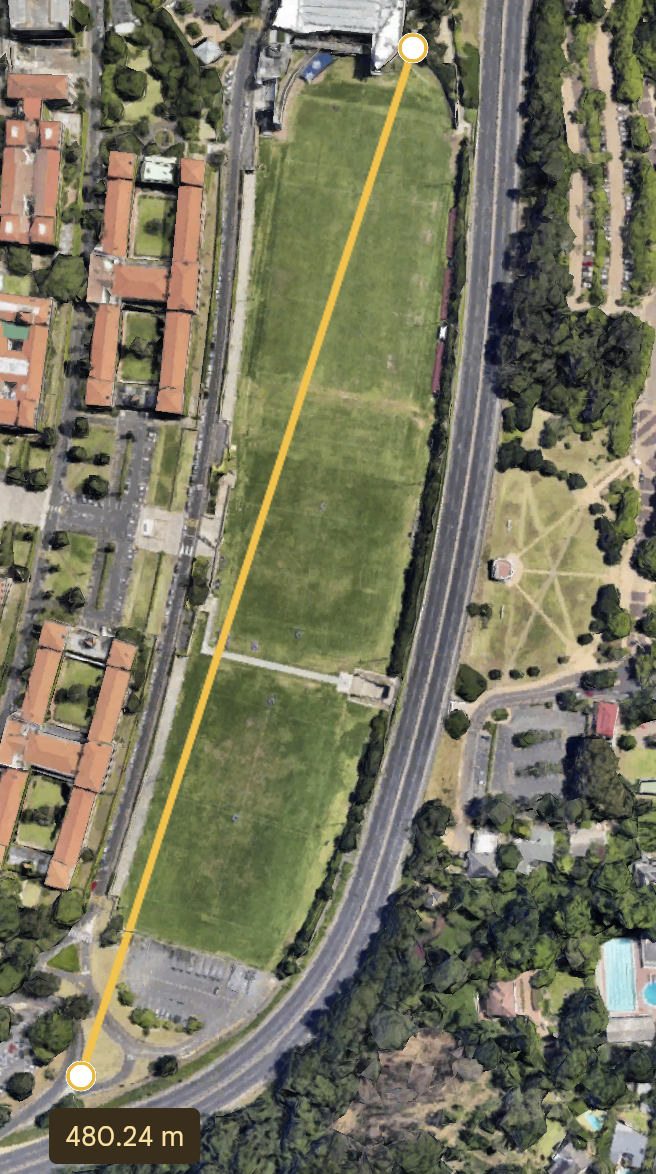
\includegraphics[width=\textwidth]{../Images/shortRangeTests/500mTestGoogleEarth.png}
        \caption{500m Test}
        \label{fig:500mtestgoogleearth}
    \end{subfigure}
    
    \caption{Short Range Rugby Field Test Distances}
    \label{fig:shortrangerugbyfieldtests}
\end{figure}

It should be noted that the 500m test was actually closer to 480m due to the physical size constraints of the rugby field itself. This was deemed as an acceptable deviation from the preferred testing distance of 500m because when compared to the larger distances that the system would be operating at, a 20m deviation from the specified testing distance is not the biggest difference and shouldn't affect results too much. For the short-range tests, all the steps described in section \ref{sec:datacollection} were followed. The two operators of the transmission and receiver systems were positioned at various distances away from each other and then performed the required tests at 100m, 300m, and 500m. Some images of the testing process can be seen below in figure \ref{fig:shortrangerugbyfieldtestphotos} below.

\begin{figure}[H]
    \centering
    \begin{subfigure}[b]{0.5\textwidth}
        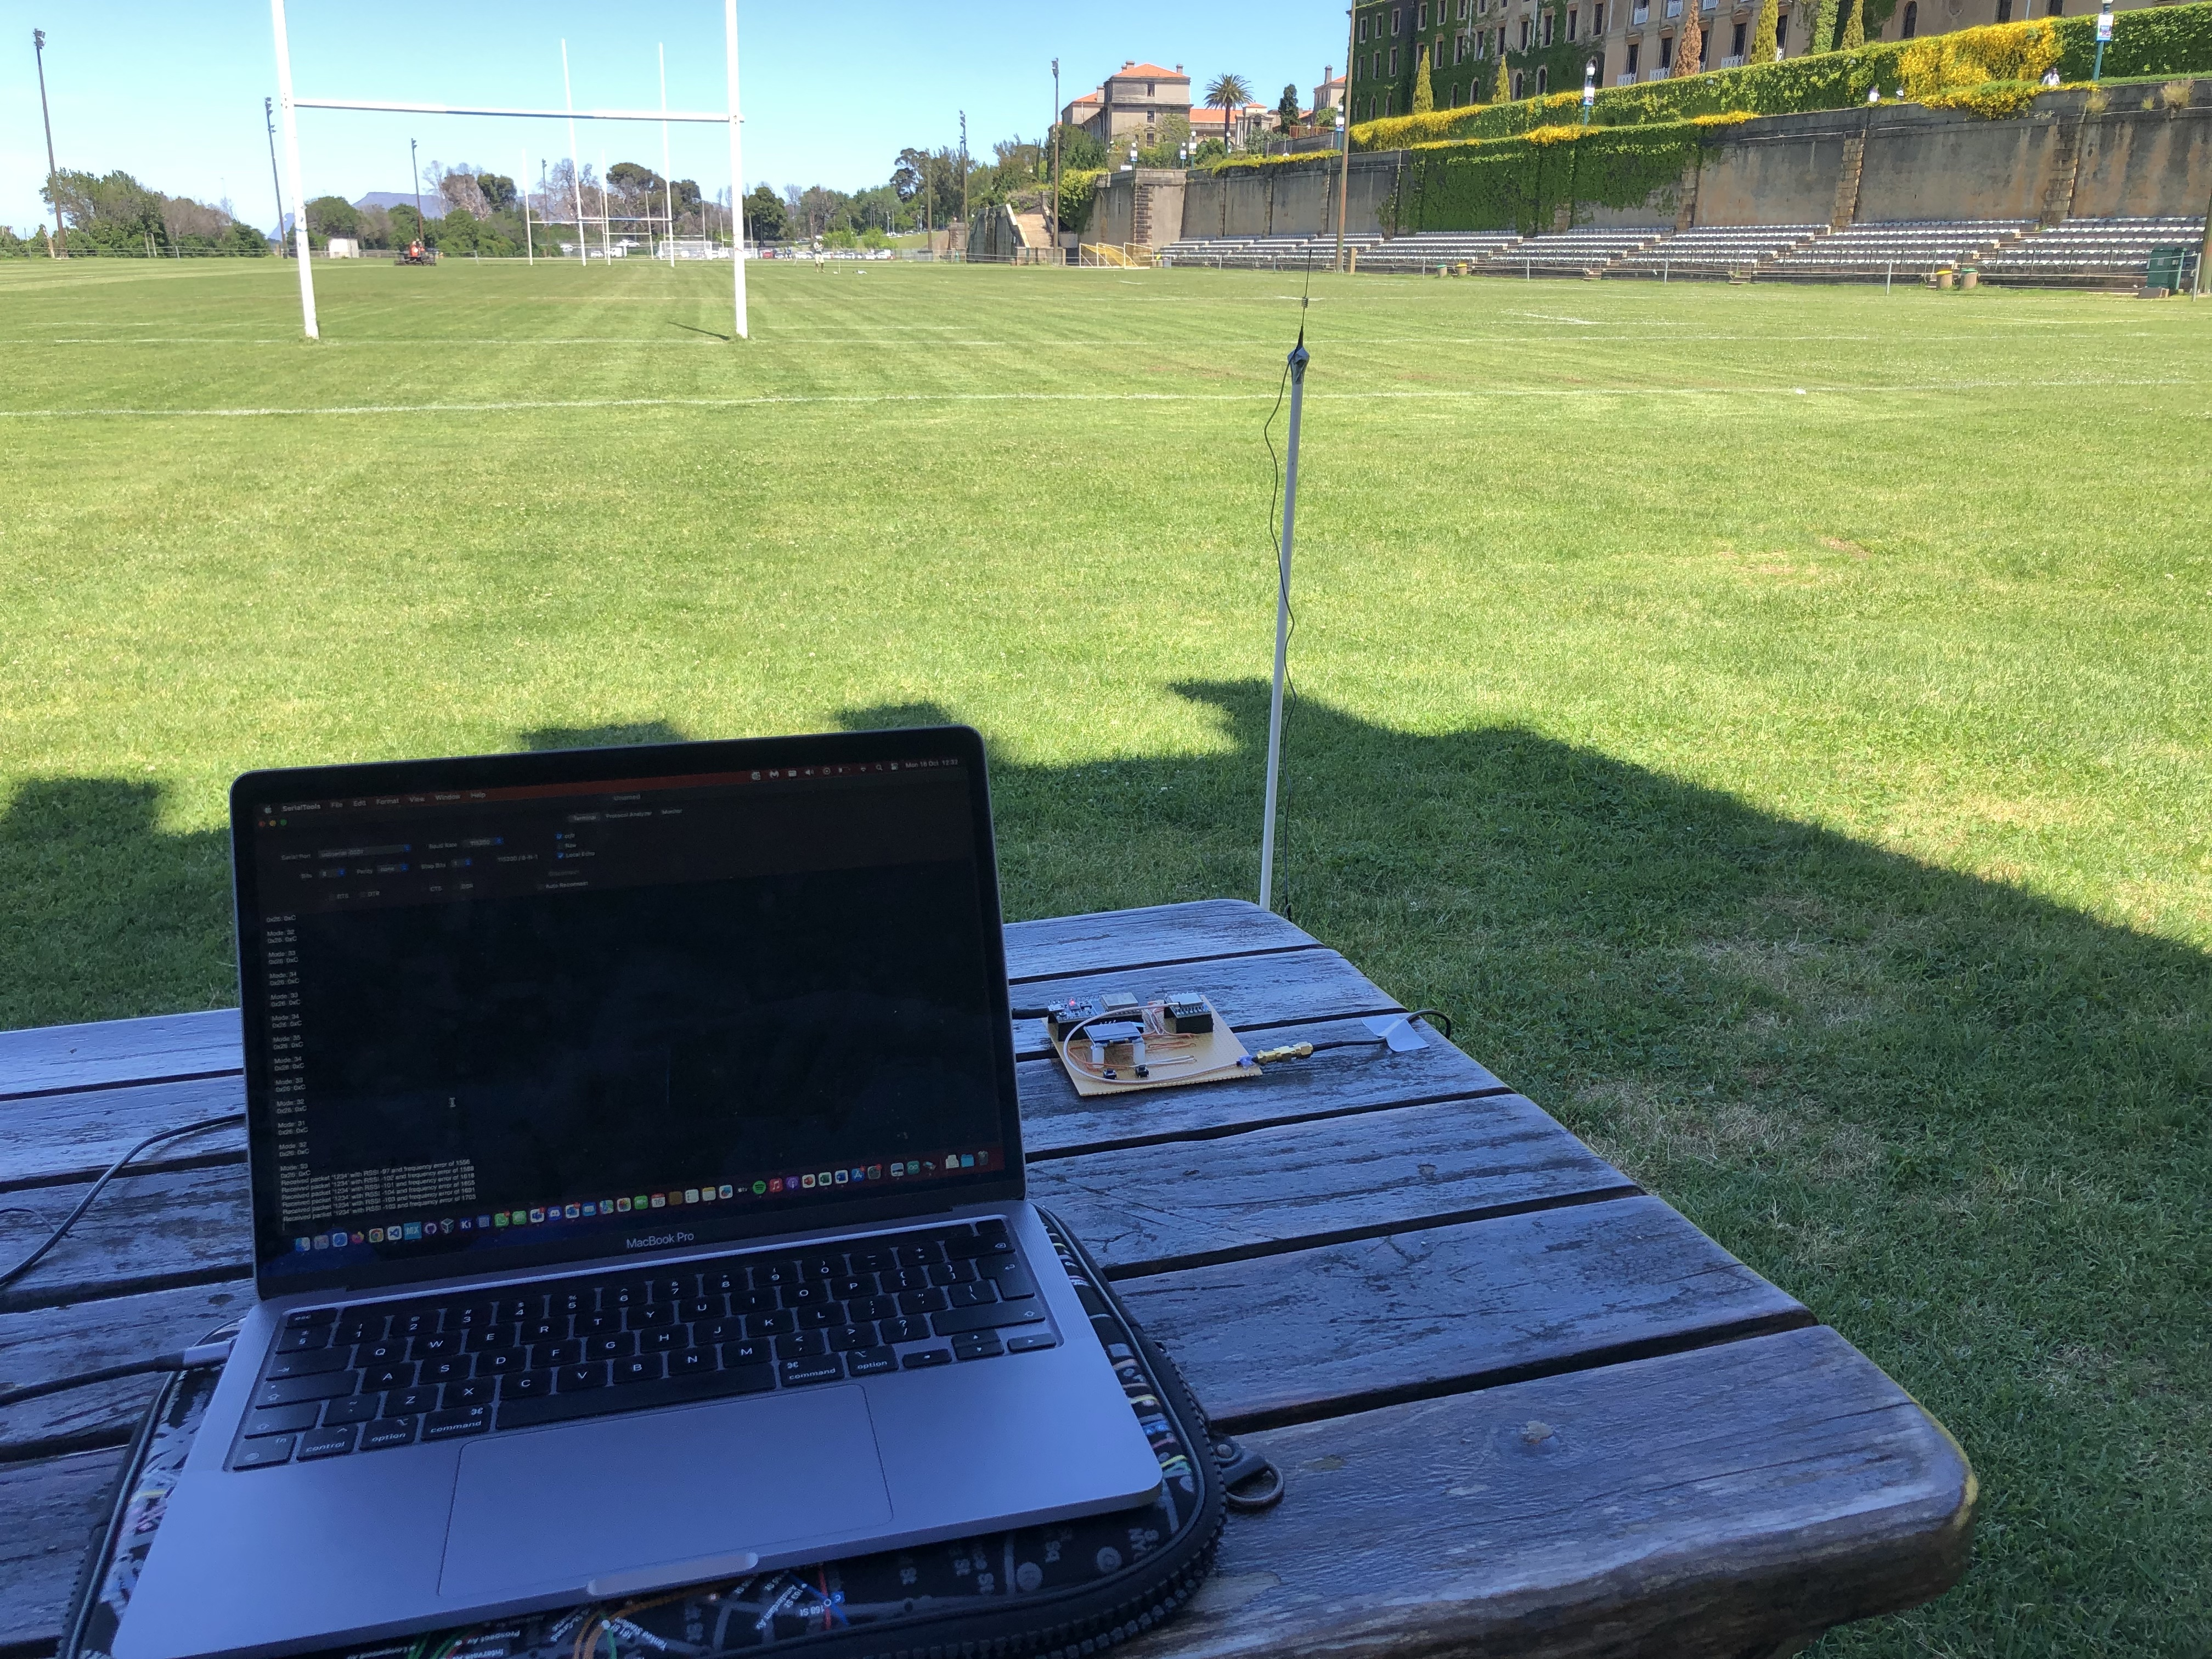
\includegraphics[width=\textwidth, valign=c]{../Images/shortRangeTests/shortRange2.jpg}
        \caption{Receiver Base Station}
        \label{fig:receiverbasestation}
    \end{subfigure}
    \hfill
    \begin{subfigure}[b]{0.35\textwidth}
        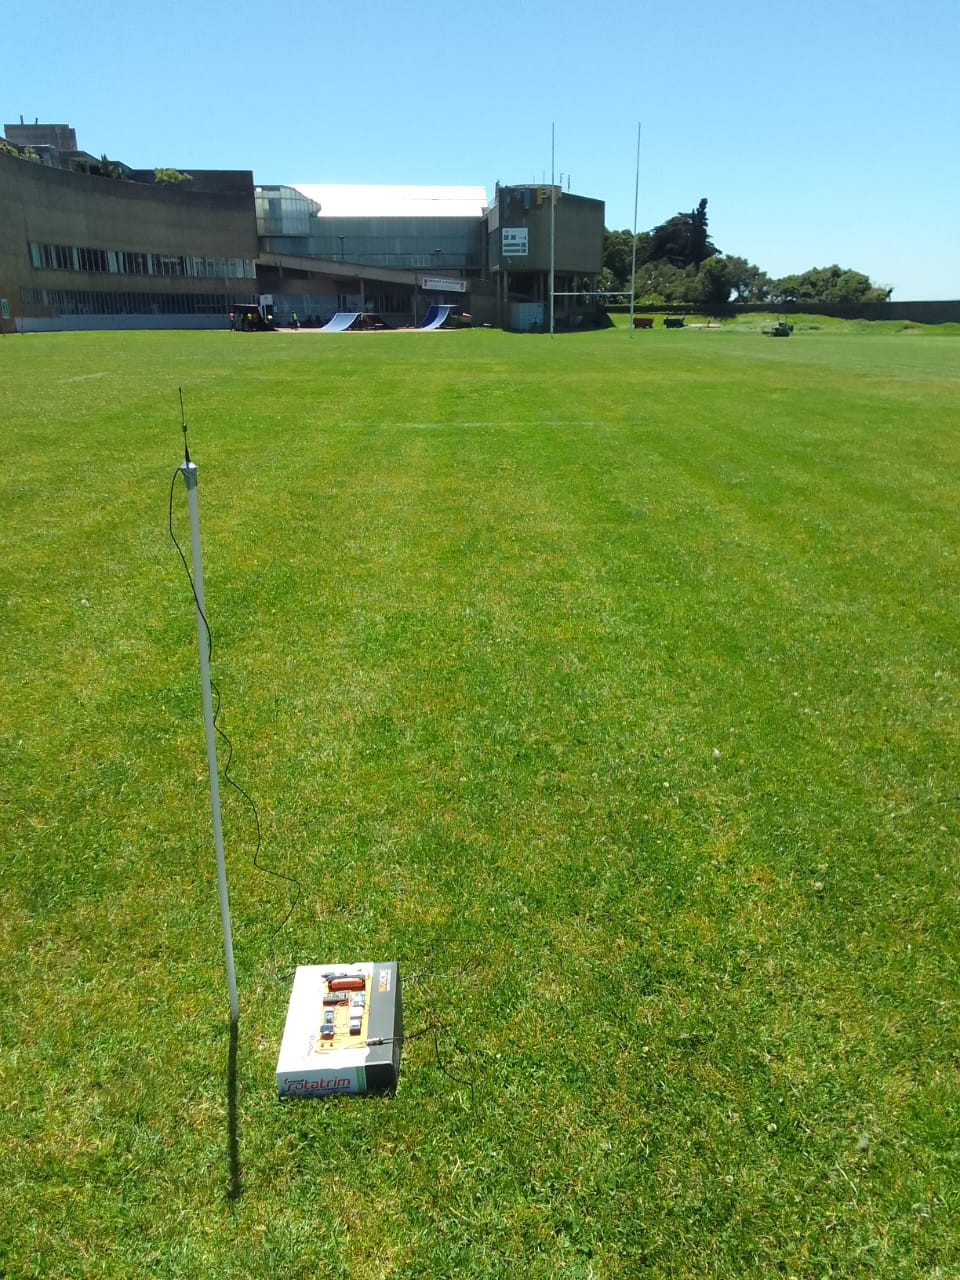
\includegraphics[width=\textwidth, valign=c]{../Images/shortRangeTests/shortRange3.jpeg}
        \caption{Transmitter Module}
        \label{fig:transmittermoduleduringtesting}
    \end{subfigure}    
    \caption{Short Range Rugby Field Testing Procedures}
    \label{fig:shortrangerugbyfieldtestphotos}
\end{figure}

The two whip antennas were placed on plastic poles so that they could be lifted off of the ground to ensure that there was no interference from the Fresnel zones interacting with the ground. Once the short-range tests were completed, the long-range test could be planned.

\section{Long-Range Test}
Since the goal of the experiments is to determine the best LoRa settings for the maximum transmission distance, it was decided that the long-range test should be suitably far to provide a realistic idea of what a real weather balloon system would have to cope with. It must be noted that, like the other tests performed, the long-range test requires a line-of-sight link between the transmitter and the receiver modules. It therefore became necessary to determine a location that would give a suitably far distance between the transmitter and receiver, while still maintaining a line-of-sight link between transmitter and receiver. The location that was decided on for the long-range test was therefore decided to be with the transmitter on Lions Head Mountain in Cape Town, and the receiver at the Tygerburg Nature Reserve in Welgemoed, Cape Town. The distance between these two points can be seen in figure \ref{fig:longrangetestdistancemap} below. 

\begin{figure}[H]
    \centering
    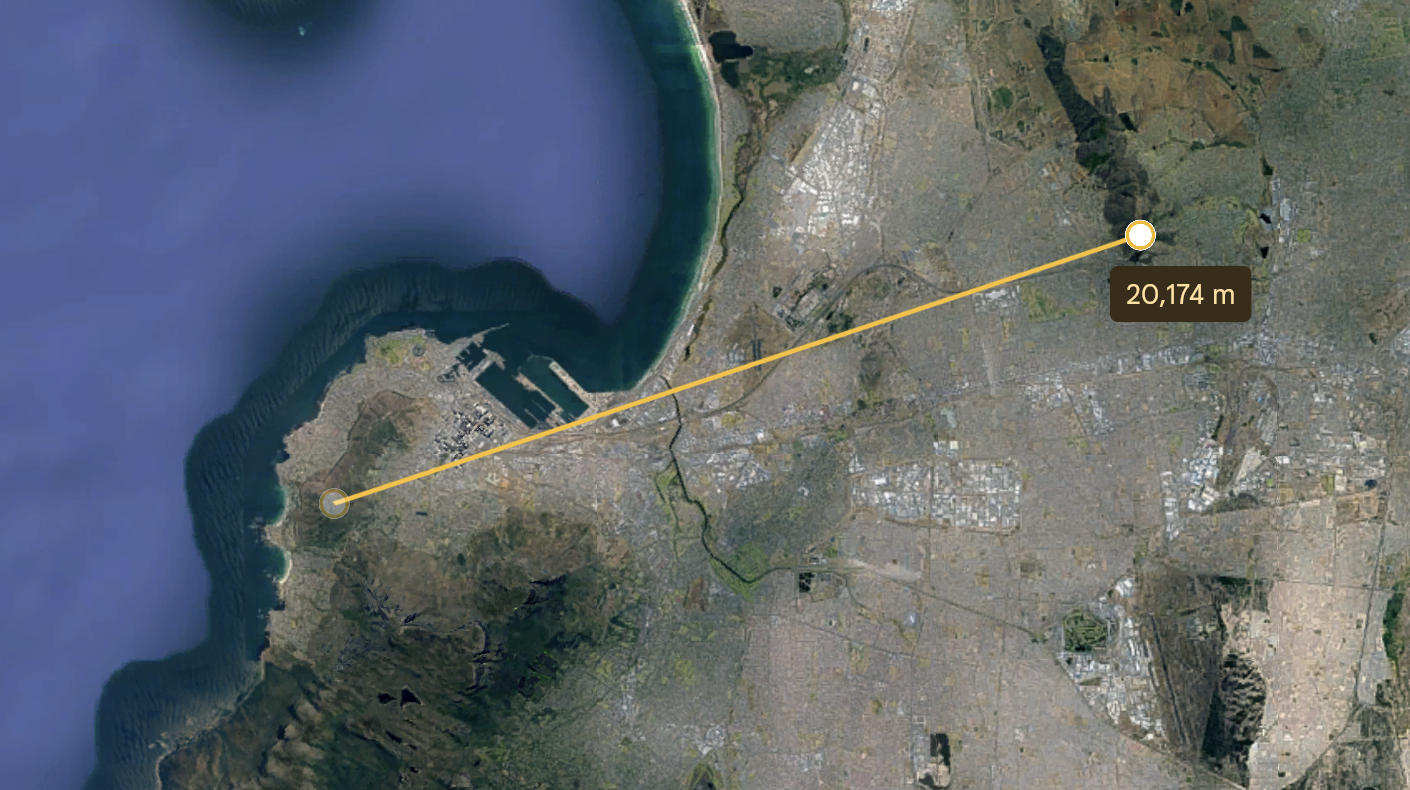
\includegraphics[width=0.65\linewidth]{../Images/longRangeTestGoogleEarth.png}
    \caption{Long Range Test Distance Map}
    \label{fig:longrangetestdistancemap}
\end{figure}

For the long-range test, it was decided that a more directional antenna should be utilised to improve the performance of the system. A dual-polarised Yagi antenna was provided to me. The reason a dual-polarised antenna had to be used was because it was the only one available from the department that was tuned to the 433MHz band of frequencies. I did however only operate the antenna in single-polarisation mode. The long-range test took place on a fairly clear day in mid-October. There was a direct line-of-sight between the transmitter on Lions Head Mountain, and the receiver on one of the hills in the Tygerburg Nature Reserve. Using equation \ref{eq:fresnelzoneradius}, one can determine the 1st Fresnel zone radius to be roughly 58.83m. This was not an issue since the transmission took place between a large mountain, and a very big hill, which meant that the halfway point wouldn't have experienced any interference within the 58.83m radius of the 1st Fresnel zone. Figure \ref{fig:transmitteronlionshead} below shows the transmitter setup on Lions Head Mountain.

\begin{figure}[H]
    \centering
    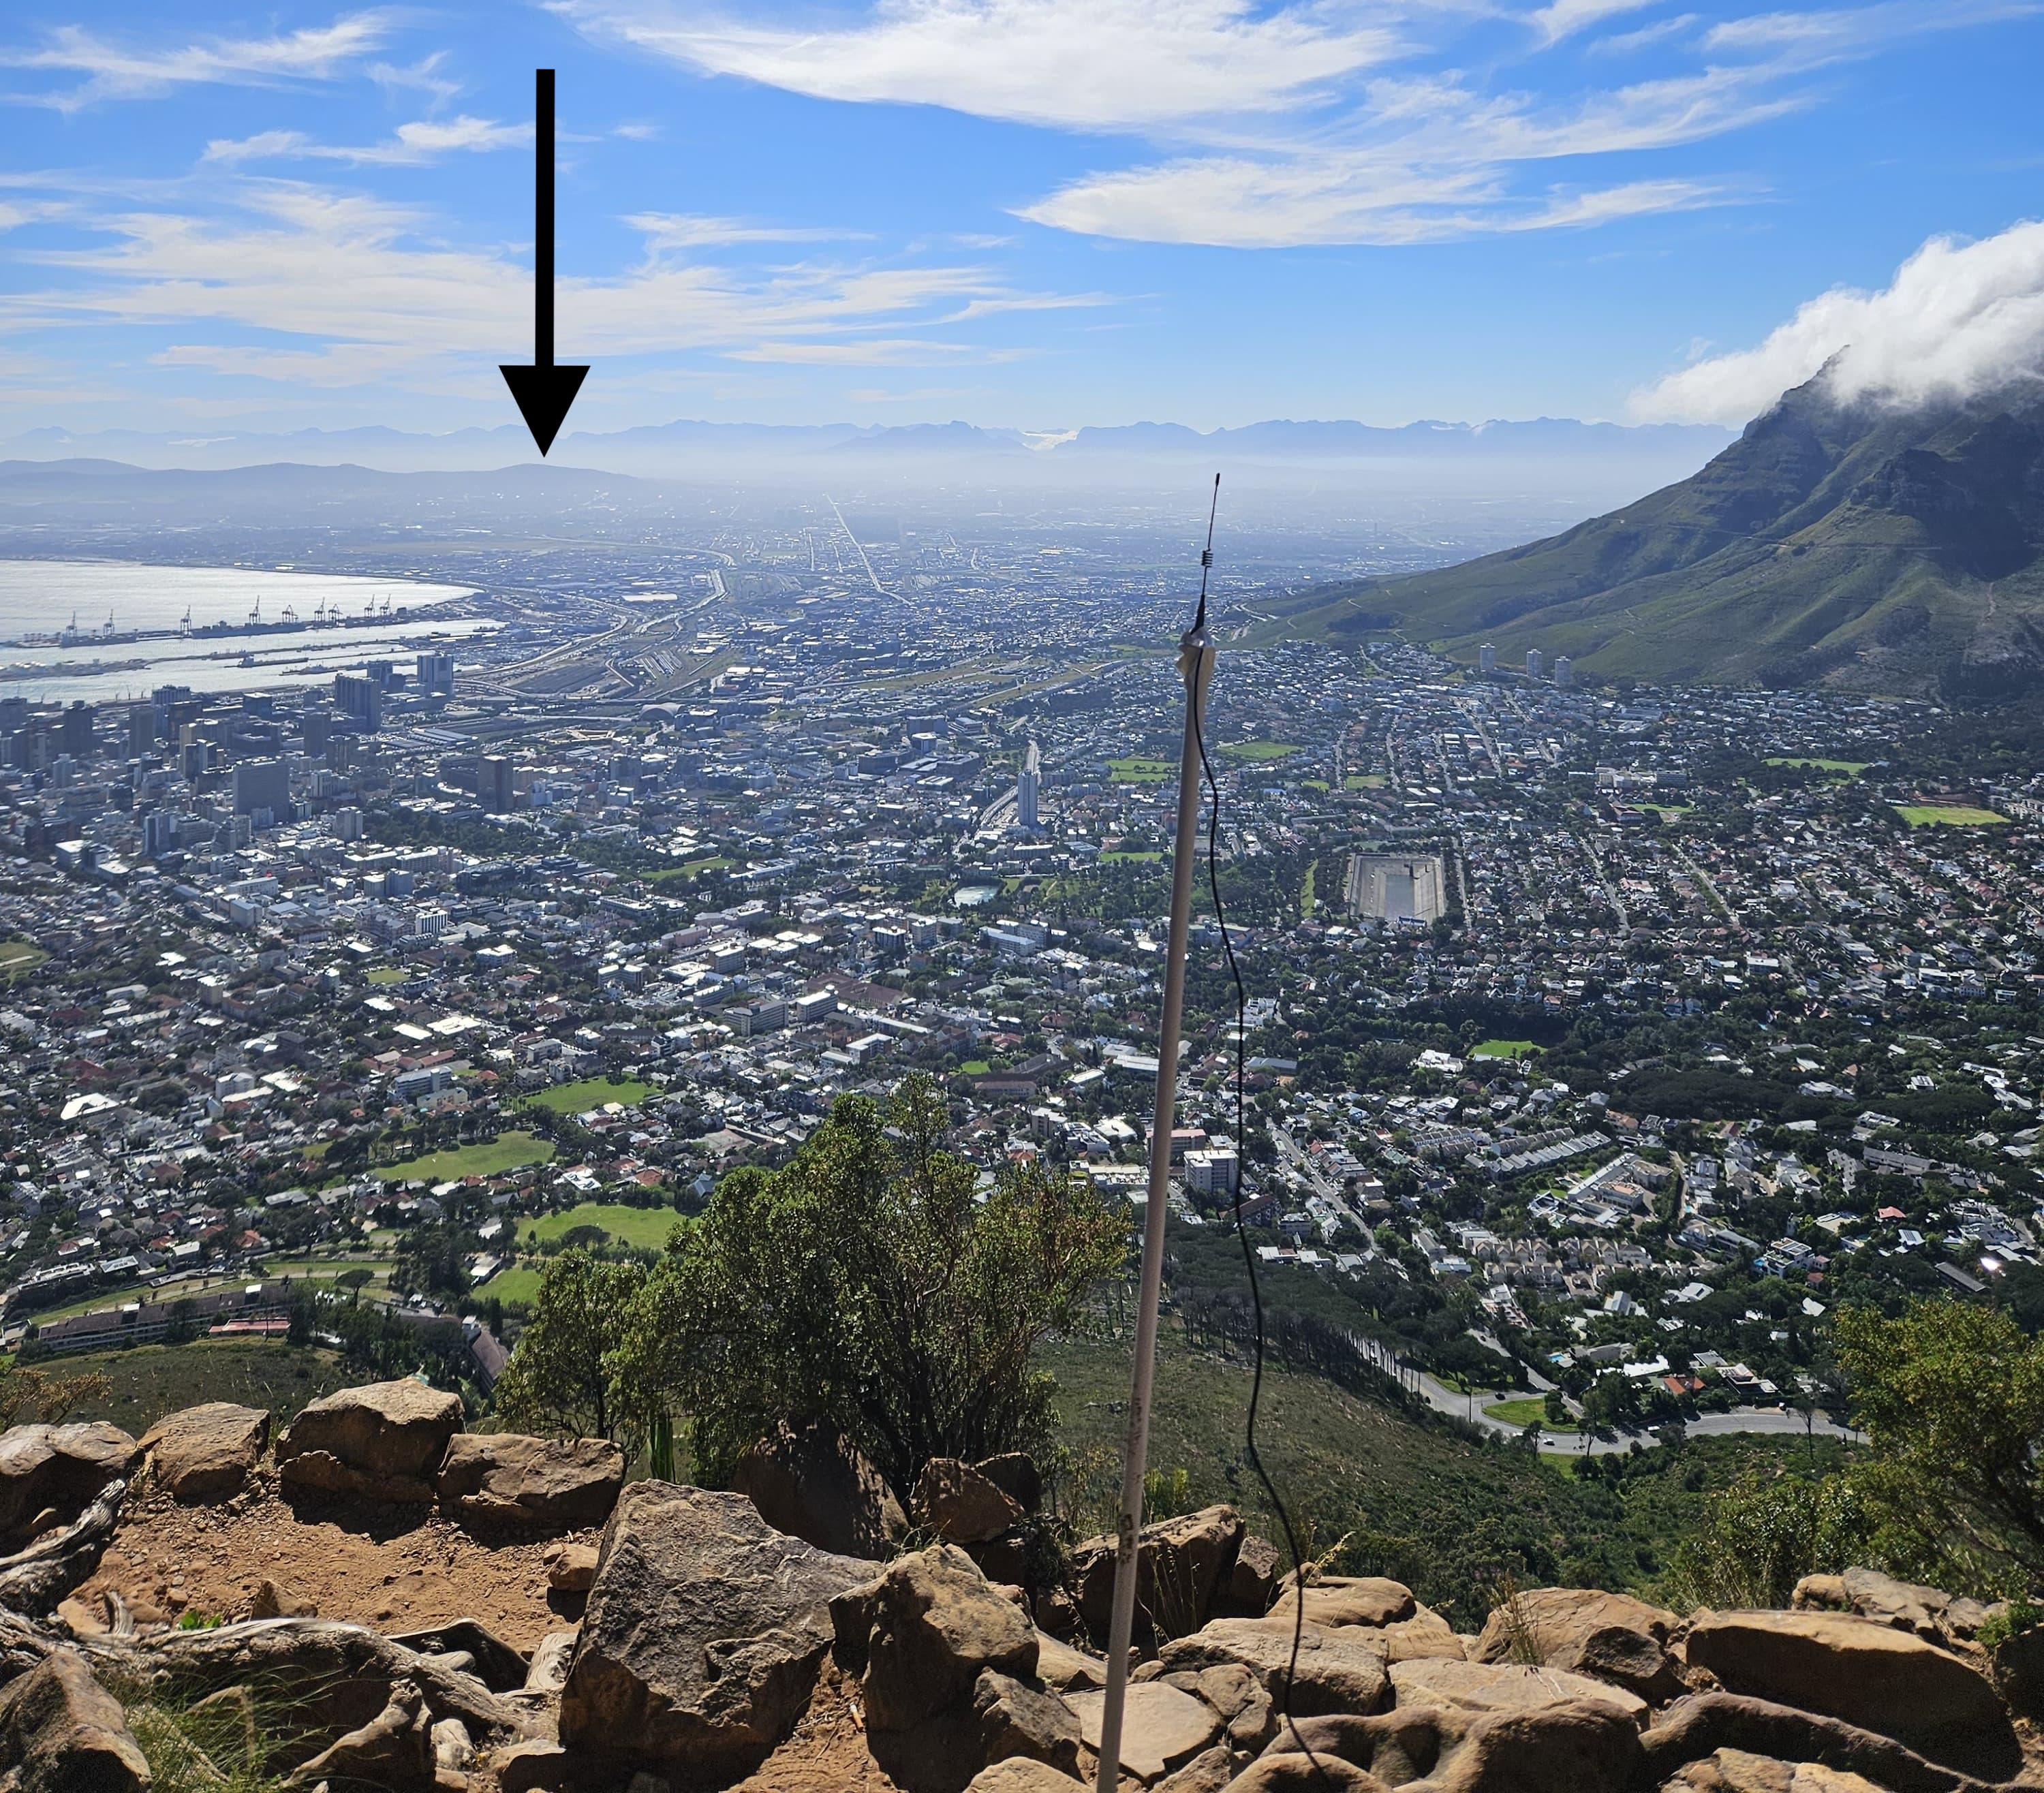
\includegraphics[width=0.6\linewidth]{../Images/longRangeTest/longRange5.jpeg}
    \caption{Transmitter Module on Lions Head}
    \label{fig:transmitteronlionshead}
\end{figure}

The black arrow indicates the position of the receiver station in the Tygerburg Nature Reserve. The receiver setup is pictured in figure \ref{fig:receivermoduleintygerburgnaturereserve} below.

\begin{figure}[H]
    \centering
    \begin{subfigure}[b]{0.4\textwidth}
        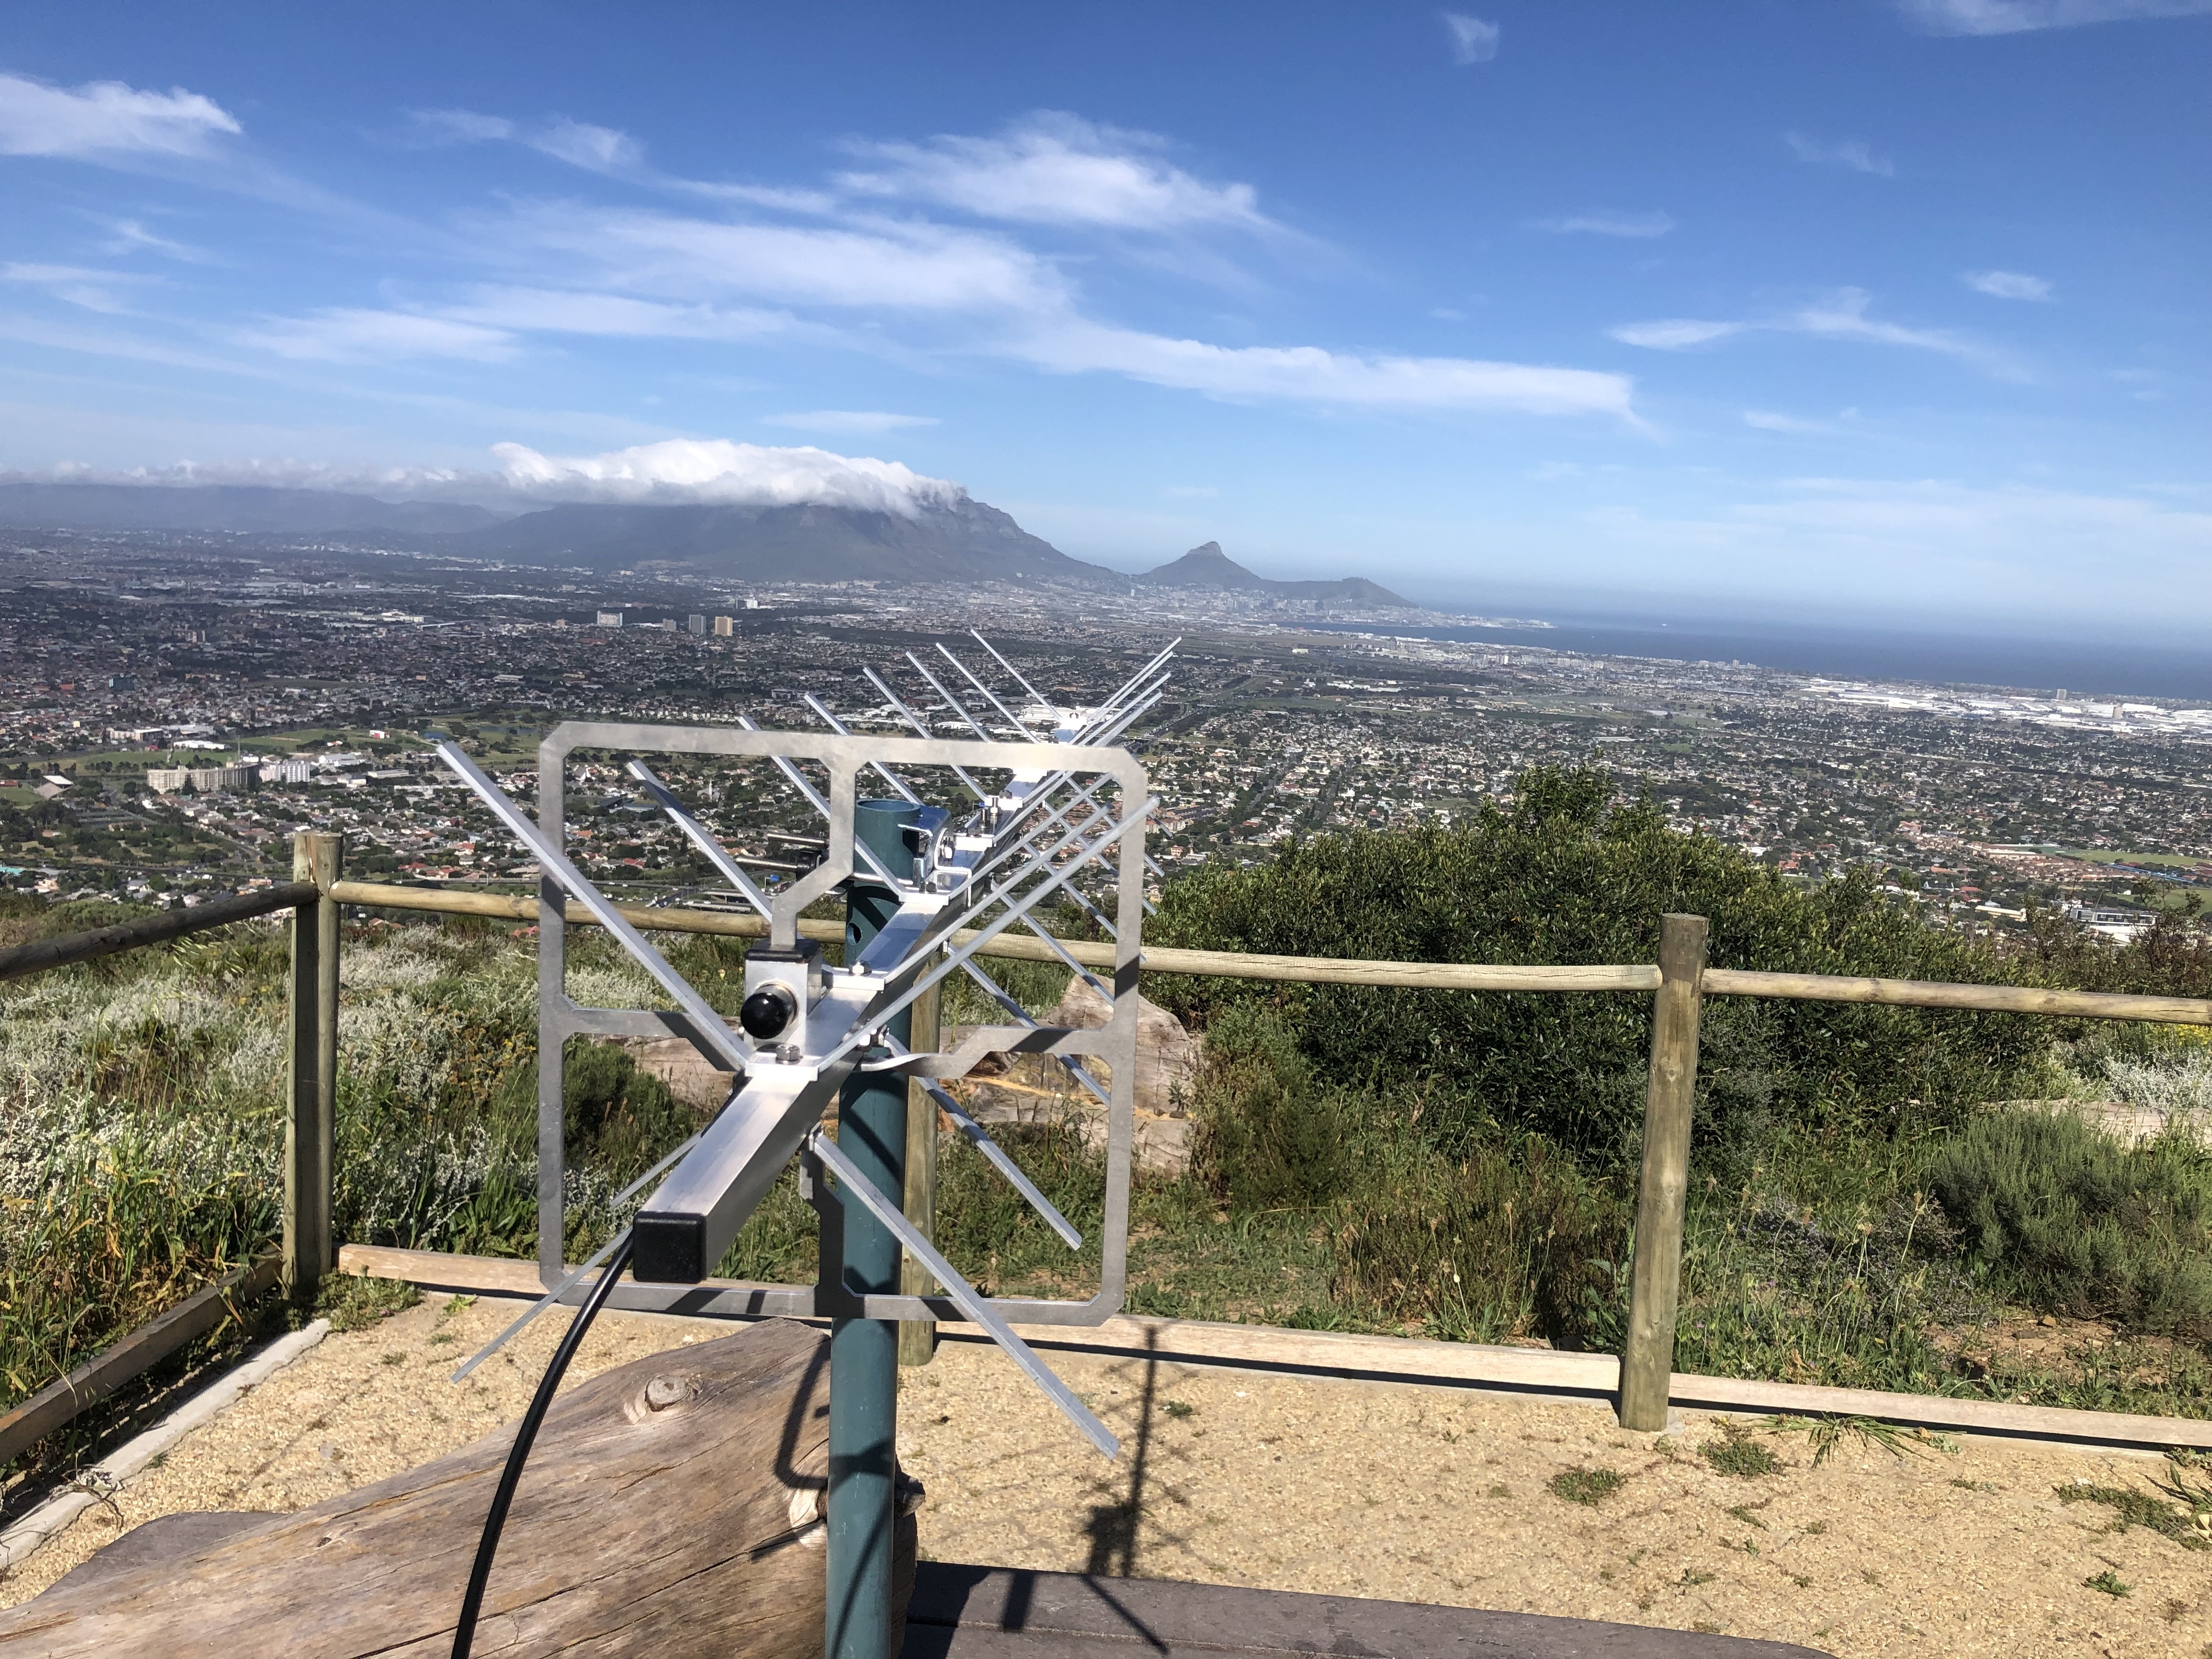
\includegraphics[width=\textwidth, valign=c]{../Images/longRangeTest/longRange1.jpg}
        \caption{Receiver Antenna Setup}
        \label{fig:receiverantennasetup}
    \end{subfigure}
    \hfill
    \begin{subfigure}[b]{0.4\textwidth}
        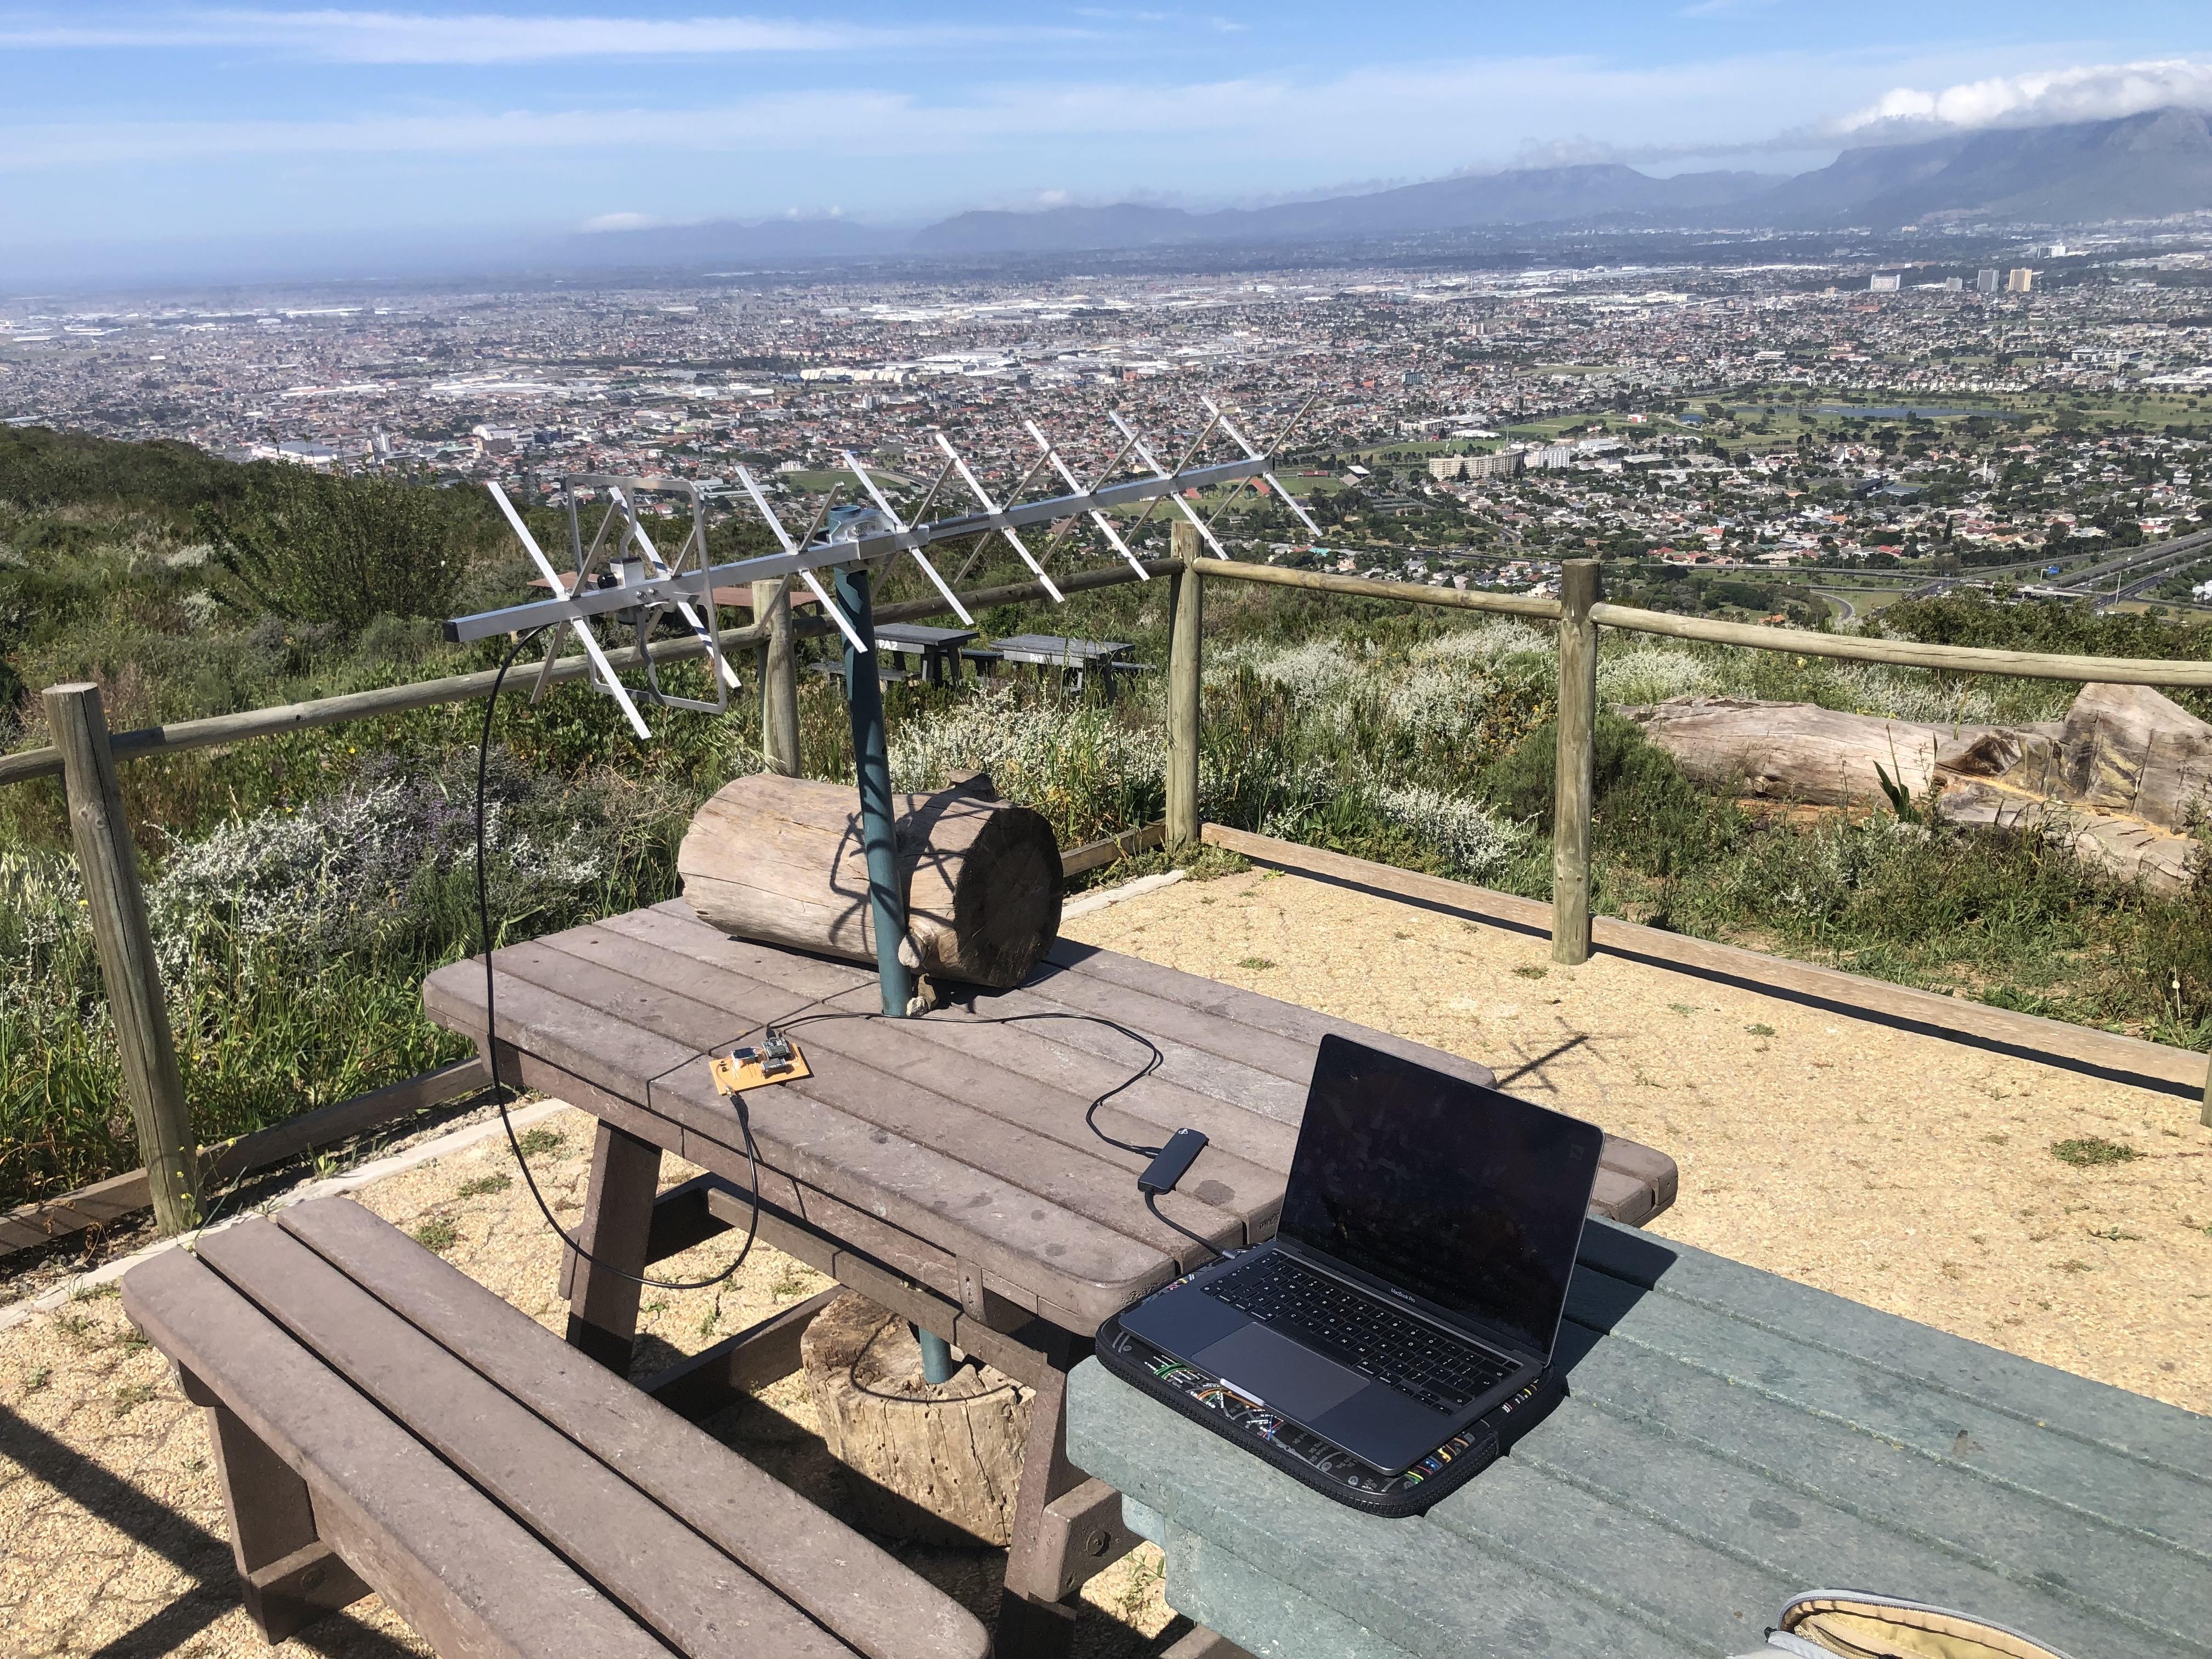
\includegraphics[width=\textwidth, valign=c]{../Images/longRangeTest/longRange3.jpg}
        \caption{Overall Receiver Setup}
        \label{fig:overallreceiversetupforlongrangetest}
    \end{subfigure}    
    \caption{Receiver Module in Tygerburg Nature Reserve}
    \label{fig:receivermoduleintygerburgnaturereserve}
\end{figure}

As you can see from the above figure, the receiver station implemented the dual polarized yagi antenna instead of the simple whip antenna used at the transmitter module. 


% ----------------------------------------------------
\ifstandalone
\bibliography{../Bibliography/References}
\printnoidxglossary[type=\acronymtype,nonumberlist]
\fi
\end{document}
% ----------------------------------------------------